\section{Forze}
%---------------------------------------------------------------------------
Se su un corpo agiscono più forze, diremo che il corpo è in equilibrio
statico se e solo se la risultante delle forze (la somma) è nulla.\\
Supponiamo di avere un corpo soggetto ad $n$ forze, se chiamiamo la
forza $i$-esima: $\vec F_i$, la risultante sarà:

\begin{equation}
    \vec F = \sum_{i=1}^n\vec F_i =  \sum_{i=1}^n m\vec a_i =
    m \sum_{i=1}^n \vec a_i\quad\mbox{eq. statico}\quad\Leftrightarrow
    \quad\vec F = \vec 0
\label{eq:forces:superposition}
\end{equation}

\subsection{Forza di reazione vincolare}
Ogni volta che un corpo soggetto ad una forza incontra un vincolo,
quest'ultimo esercita per il principio di azione e reazione un forza
uguale e opposta, in modo tale da bilanciare la forza applicata.
La forza di reazione vincolare è chiamata anche forza di reazione normale,
dato che è ortogonale al vincolo ed infatti è indicata con la lettera $\vec N$.
\begin{figure}[htbp]
    \begin{center}
        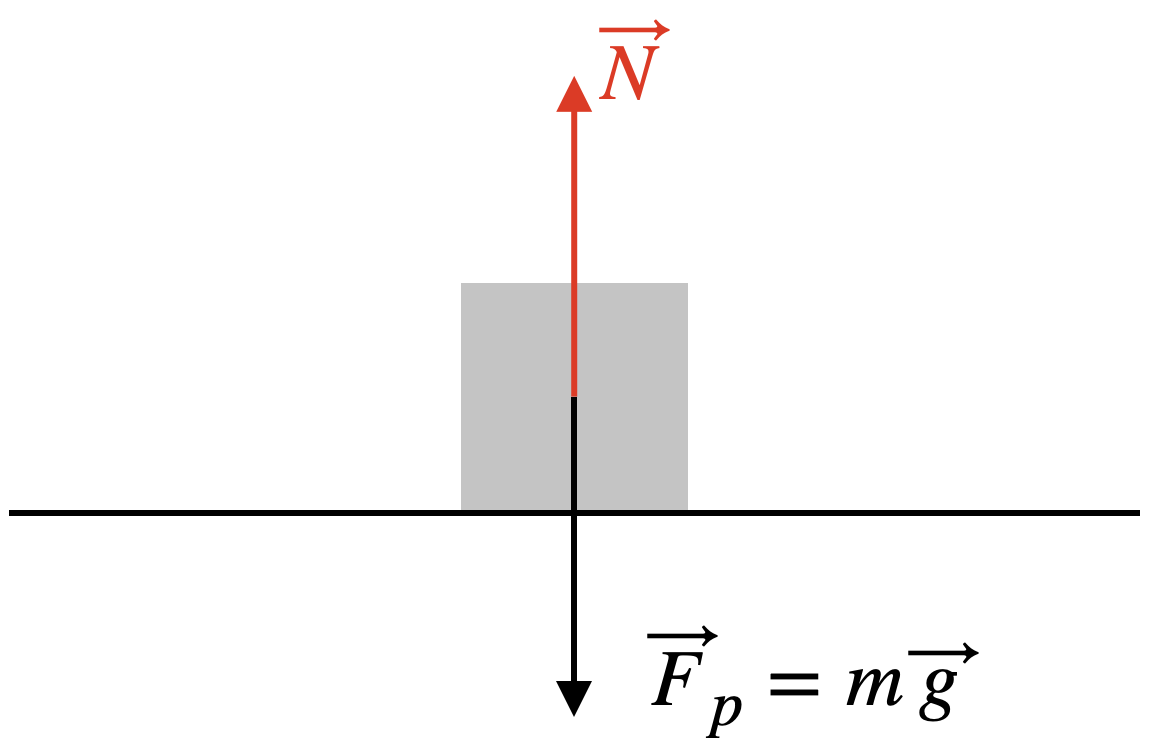
\includegraphics[width=7cm]{images/NP.png}
        \caption{Corpo in equilibrio soggetto alla forza peso ed  alla
        reazione vincolare.}
    \end{center}
\label{fig:forces:vincolar_reaction}
\end{figure}
\\
In questo caso abbiamo solo due forze, la forza peso e la forza di reazione
vincolare e sono entrambe dirette lungo la stessa direzione, ma di verso
opposto.

\begin{equation}
    \vec N + \vec F_p = \vec 0 \seg N - F_p = N - mg = 0 \seg \boxed{N = mg}
\label{eq:forces:vincolar_reaction}
\end{equation}
\\
\begin{figure}[htbp]
\center
        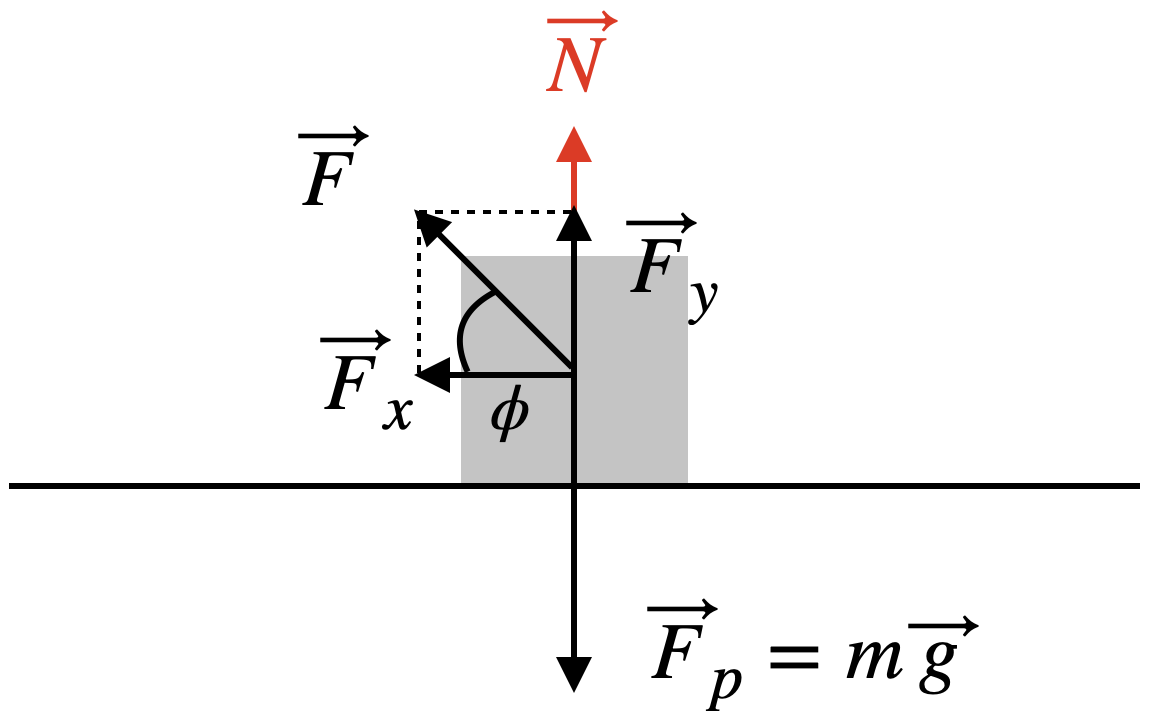
\includegraphics[width=7cm]{images/NPF.png}
        \caption{Corpo soggetto alla forza peso, alla forza $\vec F$ ed alla
        reazione vincolare.}
        \label{fig:vincolar_reaction_2}
\end{figure}
\\
Nella situazione rappresentata in figura (\ref{fig:vincolar_reaction_2}),
notiamo che l'aggiunta di una terza forza nel sistema modifica l'intensità
di $\vec N$. Per prima cosa bisogna scomporre lungo l'asse $x$ ed $y$ la
forza $\vec F$.

\begin{equation}
    \vec F = \vec F_x + \vec F_y = F_x\hat\imath + F_y\hat\jmath\seg 
    \begin{cases}
        F_x = -F\cos\phi <0\\
        F_y = F\sin\phi>0
    \end{cases}
\end{equation}
\\
Adesso procediamo con il calcolo scrivendo le equazioni di Newton.

\begin{equation}
    x:\quad F_x = m\ddot x\qquad
    y:\quad N-mg+F_y = m\ddot y = 0
\end{equation}
\\
\begin{equation}
    \mbox{Ne segue che la reazione vincolare è:}\quad \boxed{N = mg -F\sin\phi}
\end{equation}
\\
Per quanto riguarda l'asse $x$, c'è solo la componente orizzontale di
$\vec F$ che agisce sul corpo, dunque, supponendo $\phi$ ed il modulo della
forza $F$ costanti nel tempo e $\phi\ne\frac\pi2$, il corpo si muove di moto
uniformemente accelerato lungo la direzione negativa dell'asse $x$.
Con accelerazione pari a: $a = \frac{F_x}{m} = -\frac Fm\cos\phi$.

\subsection{Forze d'attrito}
Per capire cosa si una forza d'attrito consideriamo ancora il caso raffigurato
in figura (\ref{fig:vincolar_reaction_2}). La conclusione a cui siamo
giunti, ovvero che il corpo si
muove di moto uniformemente accelerato, implica l'aver considerato che non ci
sia interazione tra il corpo ed il vincolo, lungo la direzione $x$.
Inoltre è stato completamente trascurato l'effetto dell'aria sul corpo
durante il moto.
In realtà esistono tre tipi di forze, forze d'attrito, che migliorano la
descrizione del problema precedentemente trattato.\\
Le forze d'attrito radente statico e dinamico e la forza d'attrito viscoso.
\subsubsection{Attrito statico}
La forza d'attrito radente statico è la responsabile del fatto che un corpo,
posto su un piano, ha bisogno di una certa forza iniziale per cominciare il
moto. Se questo tipo di forza non esistesse basterebbe un forza piccola a
piacere per mettere un corpo in moto.\\
La forza d'attrito statico è caratterizzata dal fatto che ha un valore
variabile, da un minimo di zero, quando non si applica nessuna forza esterna,
ad un massimo che segneremo con $F_s$.
\\Dunque applicando gradualmente una forza esterna, avremo che la forza
d'attrito aumenterà anch'essa in modo graduale, bilanciando perfettamente
la forza esterna, fino al suo valore massimo.\\
Quindi ritornando al caso della figura (\ref{fig:vincolar_reaction_2})
il corpo inizia a muoversi solo se $F\cos\phi > F_s$.

\begin{equation}
    F_s = \mu_sN
\label{eq:forces:static}
\end{equation}
\\
\begin{equation}
    -F\cos\phi + F_s = -F\cos\phi + \mu_s N < 0\seg F\cos\phi >
    \mu_s\sx mg - F\sin\phi\dx
\end{equation}
\\
Dove $\mu_s$ è chiamato coefficiente d'attrito statico.
Ora supponendo di mantenere fissato l'angolo $\phi$ calcoliamo quali
valori deve assumere $F = \left|\vec F\right|$ per mettere in moto l'oggetto.

\begin{equation}
    F > \frac{\mu_s}{\mu_s\sin\phi+\cos\phi}mg
\end{equation}

\subsubsection{Attrito dinamico}
L'attrito dinamico invece entra in gioco proprio quando la forza esterna
supera il valore della forza d'attrito massima. La forza d'attrito dinamico
è una forza costante diretta in direzione opposta a quella della velocità
dell'oggetto.\\
Quindi una volta che la forza esterna supera il valore di $F_s$,
la forza d'attrito statico si annulla e si "attiva" la forza d'attrito dinamico.

\begin{equation}
    \vec F_d = -\mu_dN\hat u_v
\label{eq:forces:dynamic}
\end{equation}
\\
Supponiamo di avere una forza che soddisfi la (\ref{eq:forces:dynamic})
ne segue che:

\begin{equation}
    -F\cos\phi + \mu_dN = m\ddot x \seg \ddot x =
    \mu_dg-\frac Fm\sx\mu_d\sin\phi + \cos\phi\dx
\end{equation}
\\
L'accelerazione del corpo subisce una modifica. Trascurare l'attrito
significa considerare $\mu_{s,d}\ll 1$, ed infatti in questa approssimazione
riotteniamo il caso discusso nel paragrafo precedente, ovvero:

\begin{equation}
    F>0\quad\quad \ddot x = -\frac Fm\cos\phi
\end{equation}
\\
Un'ultima cosa da dire è che il coefficiente d'attrito statico $\mu_s$ è
sempre maggiore del coefficiente d'attrito dinamico $\mu_d$, infatti è più
facile mantenere in moto il corpo, piuttosto che spostarlo dalla sua
posizione di quiete.

\subsubsection{Attrito viscoso}
La forza di attrito viscoso è dovuto alla resistenza che oppone un fluido
quando un corpo è in movimento al suo interno. Se il fluido è in regime
laminare (non turbolento) la forza di attrito viscoso può essere stimata
con la seguente formula.

\begin{equation}
    \vec F_v = -b\vec v
\label{eq:forces:viscous}
\end{equation}
\\
Dove $b$ è il coefficiente di attrito viscoso ed è collegato alle proprietà
geometriche del corpo ed alla viscosità del fluido in questione.

\begin{equation}
    b = k\eta
\label{eq:forces:viscous_coefficient}
\end{equation}
\\
Dove $\eta$ è la viscosità del fluido, ha le dimensioni di una pressione per
un tempo $(Pa \cdot s) =(N\cdot m^{-2}\cdot s)$. Mentre $k$ è il fattore
geometrico che dipende dalla forma del corpo ed è misurato in metri, ad
esempio per una sfera $k = 6\pi R$.
Se sul corpo non agiscono altre forze oltre a quella d'attrito viscoso,
allora abbiamo anche un'accelerazione proporzionale alla velocità e dunque
un moto smorzato esponenzialmente, come quello incontrato nel paragrafo (\ref{section:MRSE}).

\begin{equation}
    \vec F_v = -k\eta\vec v = m\vec a \seg
    \vec a = -\frac{k\eta}m\vec v =-\beta \vec v 
\end{equation}
\\
È interessante considerare il caso di caduta libera in presenza di attrito
viscoso. Scegliamo un sistema di riferimento unidimensionale rivolto verso
il basso, e lasciamo cadere un oggetto a partire dall'origine.
\begin{figure}[htbp]
    \begin{center}
        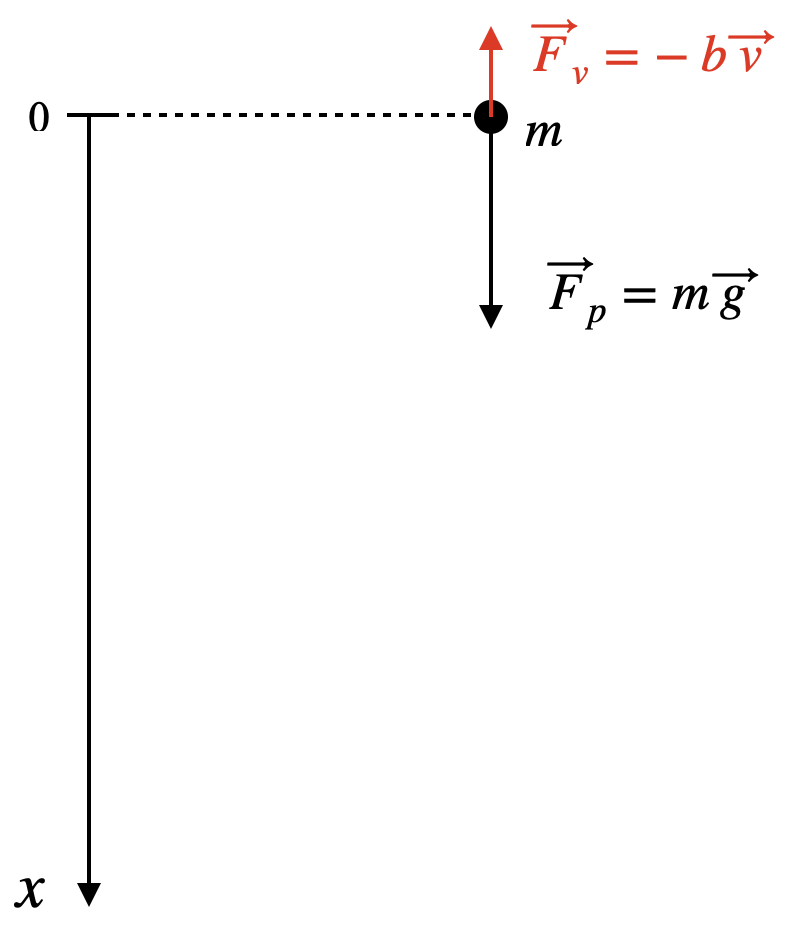
\includegraphics[width=7cm]{images/cadlibera.png}
        \caption{Corpo di massa $m$ soggetto alla forza peso ed
        alla forza di attrito viscoso.}
\end{center}
\label{fig:forces:freefall}
\end{figure}
\\
Quindi scrivendo la somma delle forze che agiscono su $m$ otterremo:

\begin{equation}
    mg - bv = m\dot v \seg \dot v = g - \frac{b}{m}v
\end{equation}
\\
Ora definiamo un tempo caratteristico del sistema, che chiameremo $\tau$.
Questo fattore determina una scala temporale del moto. La regione in cui
$t\gg\tau$ è chiamata regime, mentre la zona in cui $t\gg\tau$ è chiamata
transiente.

\begin{equation}
    \boxed{\tau \coloneqq \frac{m}{b} = \frac1\beta}
\label{eq:forces:time_constant}
\end{equation}
\\
Andiamo ora a ricavare la velocità in funzione del tempo.

\begin{equation}
    \dot v = g - \frac bmv = g - \frac v\tau = -\frac1\tau\sx v - g\tau\dx
    \seg \frac{\dot v}{v -g\tau} = -\frac1\tau
\end{equation}
\\
\begin{multline}
   \int_0^{v_{(t)}}\frac{d v}{v -g\tau} = -\int_0^t\frac{dt'}\tau\seg
   \ln\sss 1 - \frac{v_{(t)}}{g\tau}\ddd = -\frac t\tau\seg
   \\\seg\boxed{v_{(t)} = g\tau\sx1-e^{-\frac t\tau}\dx}
\label{eq:forces:viscous_v}
\end{multline}
\\
Integrando nuovamente si ottiene l'equazione del moto:

\begin{equation}
    x_{(t)} = g\tau\int_0^tdt'\sx1-e^{\frac{-t'}\tau}\dx \seg
    \boxed{x_{(t)} = g\tau\sss t + \tau\sx e^{-\frac t\tau} - 1\dx\ddd}
\label{eq:forces:viscous_x}
\end{equation}
\\
\begin{figure}[htbp]
\center
        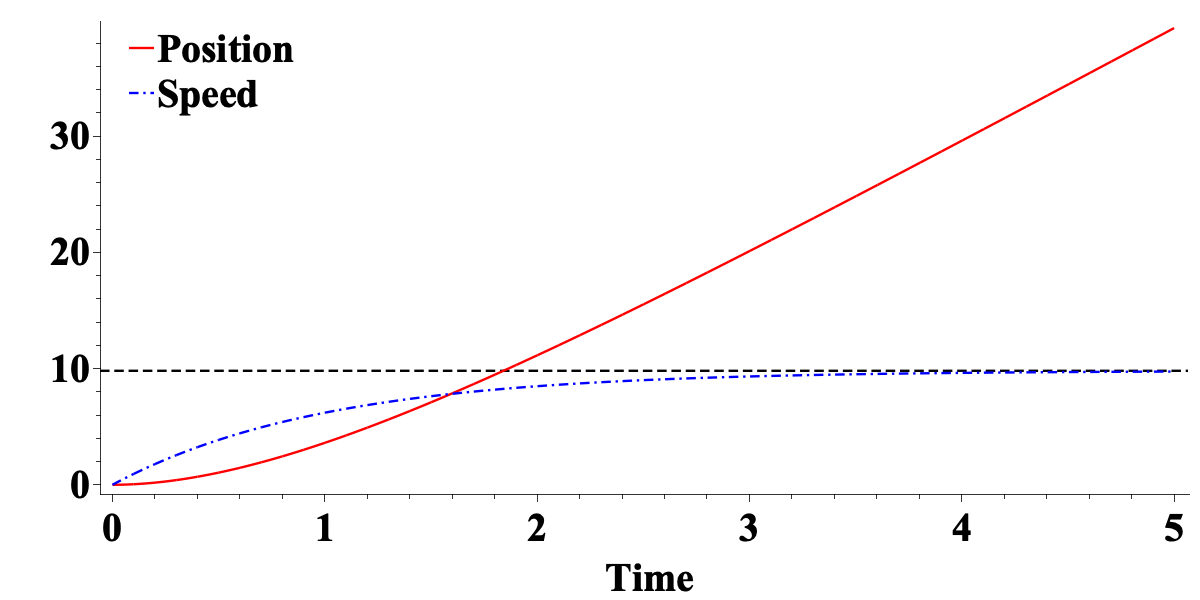
\includegraphics[width=13cm]{images/freefallXV.png}
        \caption{Spazio percorso (rosso) e velocità (blu) di un corpo in
        caduta libera con attrito viscoso. La linea orizzontale tratteggiata
        rappresenta il valore asintotico (a regime) della velocità.
        L'asse delle ascisse rappresenta il tempo in unità di $\tau$.}
\label{fig:forces:freefall:curves}
\end{figure}
\\
Il valore a regime di $v_{(t)}$ si calcola facendo il limite per
$t\gg\tau\seg$

\begin{equation}
    v_\infty\coloneqq v_{\sx t\gg\tau \dx} = g\tau
\label{eq:forces:viscous_vlim}
\end{equation}
\\
La velocità tende a diventare costante in quanto la forza d'attrito tende a
bilanciare la forza peso dunque il corpo tenderà a muoversi di moto
rettilineo uniforme.\\
Se invece sviluppiamo sia $x_{(t)}$ che $v_{(t)}$ per $t\ll\tau$,
possiamo osservare che l'effetto della forza d'attrito è ancora troppo
piccolo e quindi le curve posso essere approssimate con le equazioni della
caduta libera senza attrito.\\
Le leggi orarie della posizione e della velocità, ed anche la velocità di regime
sono rappresentate in figura (\ref{fig:forces:freefall:curves}). Nelle figure
(\ref{fig:freefall_approx_x}) e (\ref{fig:freefall_approx_v})
abbiamo messo in risalto la differenza tra le soluzioni con attrito e quelle
senza attrito.

\begin{figure}[htbp]
    \center
    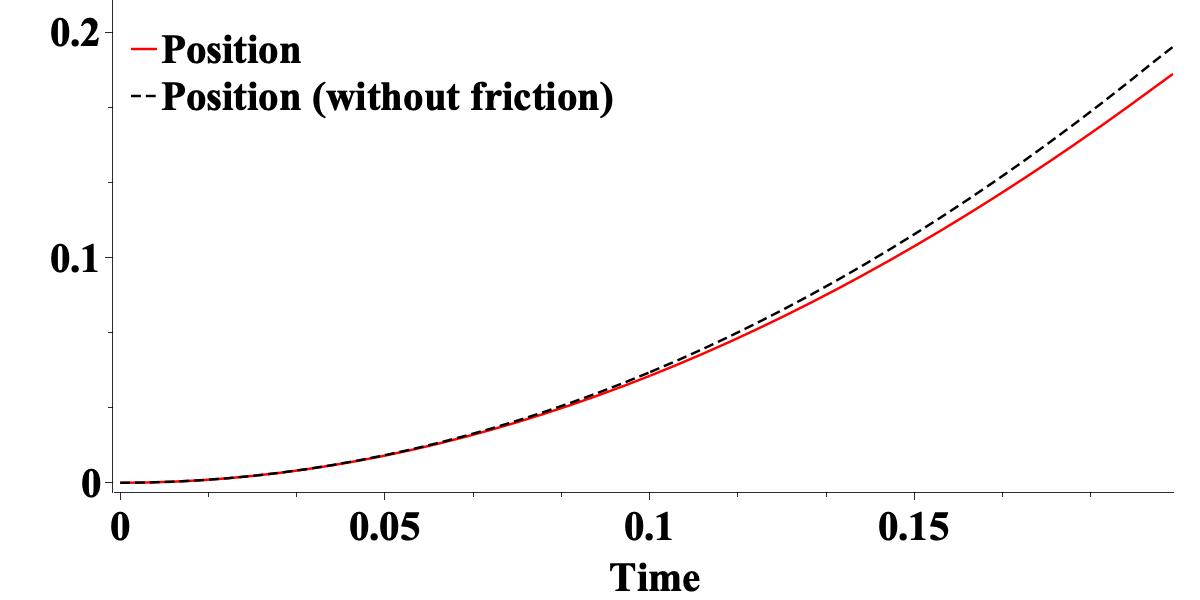
\includegraphics[width=13cm]{images/freefallX.png}
    \caption{Approssimazione per piccoli tempi, la curva nera è l'equazione
    della posizione in funzione del tempo in caduta libera senza attrito:
    $x_{(t)} = \frac12gt^2$}
\label{fig:freefall_approx_x}
\end{figure}

\begin{figure}[htbp]
\center
    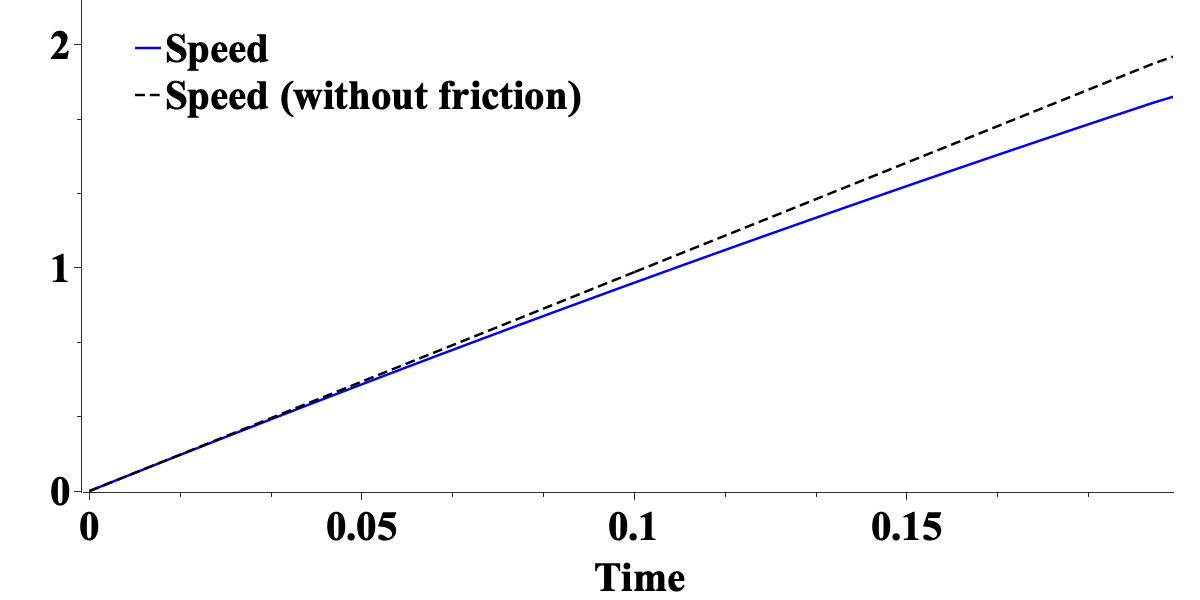
\includegraphics[width=13cm]{images/freefallV.png}
    \caption{Approssimazione per piccoli tempi, la curva nera è l'equazione
    della velocità in funzione del tempo in caduta libera senza attrito:
    $v_{(t)} = gt$}
\label{fig:freefall_approx_v}
\end{figure}

\subsection{Forza elastica}
La forza elastica è una forza di richiamo generata da una molla, quando viene
discostata dalla sua posizione di equilibrio. Essa è proporzionale alla
contrazione/dilatazione effettuata.\\ Quindi se supponiamo di avere un un
punto collegato ad una molla in posizione iniziale $\vec x_0$, e lo spostiamo
fino al punto $\vec x$, allora la forza elastica sarà:

\begin{equation}
    \vec F_e = -k\sx\vec x-\vec x_0\dx = -k\Delta x\cdot\hat u_x
\end{equation}
\\
\begin{figure}[htbp]
    \begin{center}
        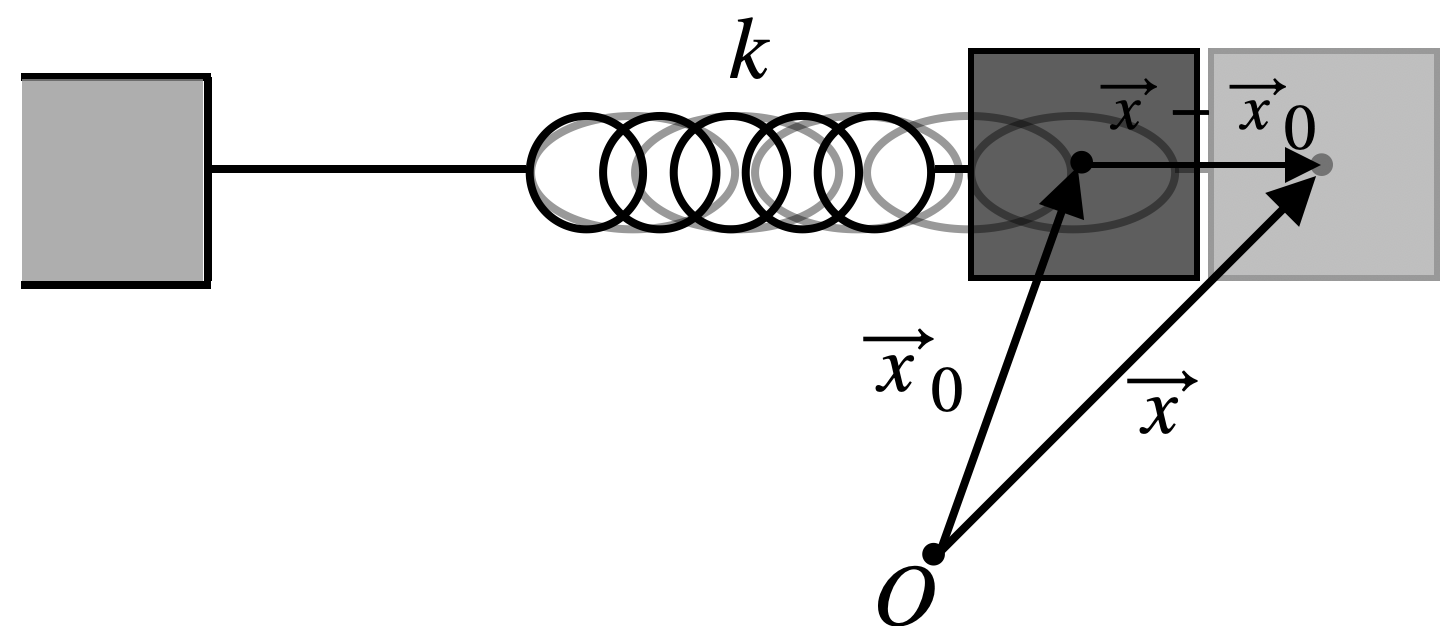
\includegraphics[width=10cm]{images/molla.png}
        \caption{Rappresentazione dell'elongazione di una molla rispetto
        alla sua posizione di riposo.}
\end{center}
\label{fig:forces:elastic}
\end{figure}
\\
La costante elastica $k$ è caratteristica della molla ed è misurata in
$\frac Nm$. Se studiamo il caso dinamico in cui un corpo è soggetto alla
sola forza elastica otterremo che:

\begin{equation}
    F_x = m\ddot x = -kx \seg \boxed{\ddot x +\frac km x = 0}
\label{eq:forces:elastic_ODE}
\end{equation}
\\
È l'equazione differenziale dell'oscillatore armonico con
$\omega = \sqrt{\frac km}$ e periodo $T =2\pi\sqrt{\frac mk}$.
La soluzione sarà come la (\ref{eq:MA}), possiamo utilizzare la funzione
coseno in quanto il punto parte da una posizione pari a $\Delta x$:

\begin{equation}
    x_{(t)} = \Delta x \cos\sx \sqrt{\frac km}t\dx
\label{eq:forces:elastic_x}
\end{equation}
\\
In realtà non è necessaria la presenza di una molla per avere una forza
elastica, e quindi questo tipo di moto, ma qualsiasi sistema fisico in cui è
presente una forza come quella in (\ref{eq:forces:elastic_ODE}) è
riconducibile ad un oscillatore armonico semplice.